\chapter{Simulations}

\section{Simulator}

A simulation environment for the USV has been set up in ROS Melodic and Gazebo 9. The simulator supports altering of the system matrices and thruster configuration. Simulated input can be provided from several sensors, including GNSS, IMU, and 2D lidar. The surrounding environment can be modified by adding and removing obstacles. The simulator is based on the Virtual RobotX simulator \citep{website:vrx}, and the theory of its operation is available in \citet{website:vrx_to}.

\section{Map generation with SLAM}

\figref{fig:sim_sensor_fusion}b shows the map generated by Cartographer after moving the USV along the edges of the area in \figref{fig:sim_sensor_fusion}a. The middle of the map is unknown due to the lidar's inability to detect across the middle.

\begin{figure}[h!]
    \centering
	\makebox[\linewidth][c]{
	\begin{subfigure}[b]{0.5\textwidth}
		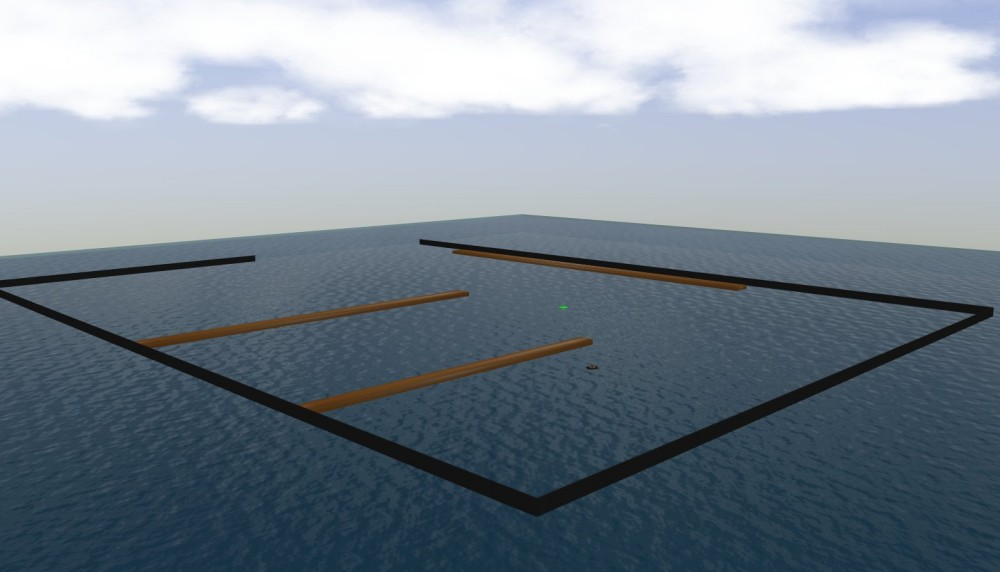
\includegraphics[width=1.0\textwidth,height=0.185\textheight]{fig/simulations/env2}
		\caption{}
	\end{subfigure}
	\begin{subfigure}[b]{0.5\textwidth}
		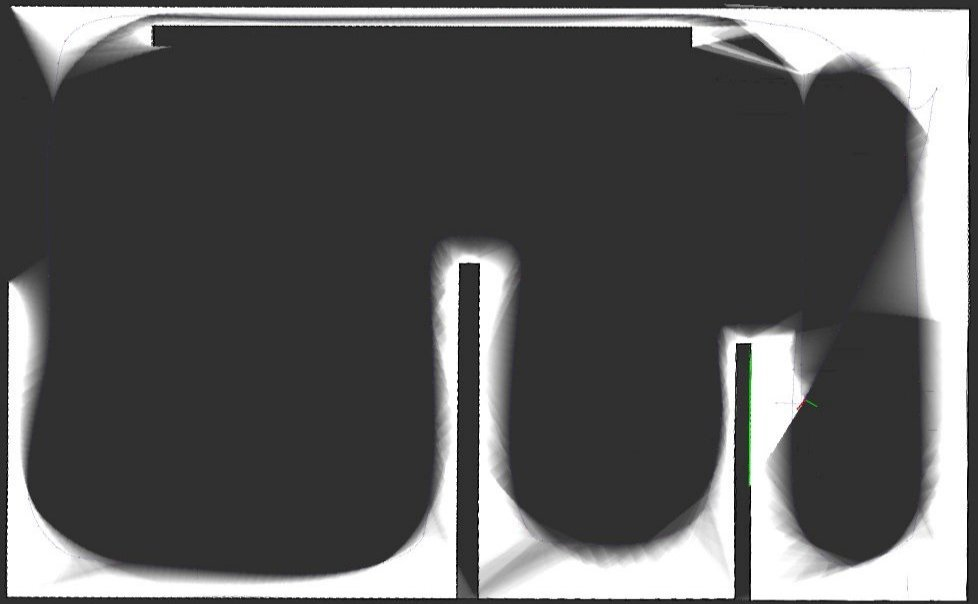
\includegraphics[width=1.0\textwidth]{fig/simulations/env_slam2}
		\caption{}
	\end{subfigure}
	}
	\caption[Map generation with SLAM of a simulated environment.]{(a) Simulation environment. (b) SLAM map. The white area of the map represents free space, the black area represents obstacles, and the dark gray area in the middle is unknown. The black area is hard to see, but is located at the most distinct transitions from white to dark gray.}
	\label{fig:sim_sensor_fusion}
\end{figure} 

\section{Complete coverage maneuvering with boustrophedon motions}

\subsection{Constant coverage range} \label{sec:sim1}

The target region and surrounding environment for this simulation is shown in \figref{fig:target_region_bm_1}. A symmetric constant coverage range of $\SI{10}{\meter}$  is assumed for the MBES, i.e. $\SI{5}{\meter}$ in both starboard and port directions. The simulated lidar has a range of $\SI{25}{\meter}$, which is the same as the lidar in the real-world experiments.

\begin{figure}[h!]
	\centering
	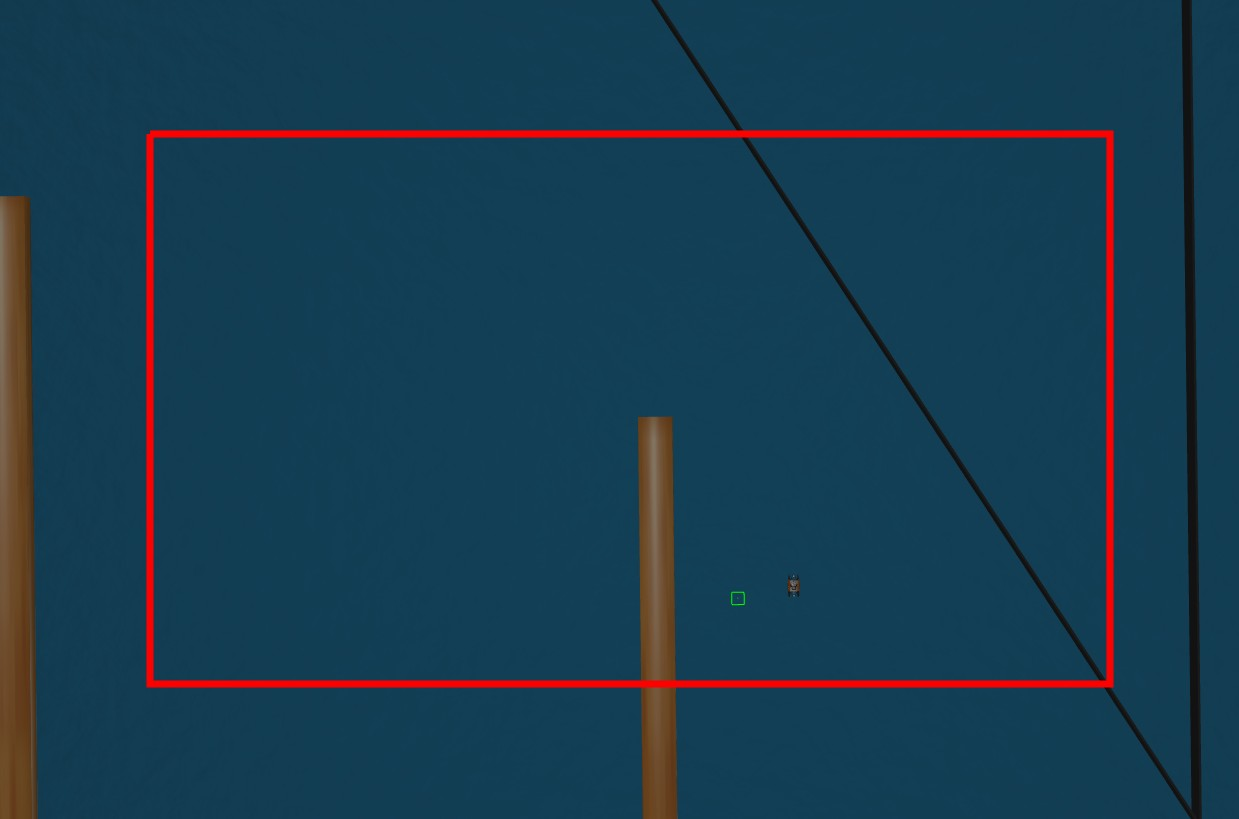
\includegraphics[width=0.7\textwidth]{fig/simulations/target_region_bm_1}
	\caption[The surrounding environment and target region for the first simulation.]{The surrounding environment and target region for the first simulation. The USV is depicted at its starting position.}
	\label{fig:target_region_bm_1}
\end{figure}

The following parameters were used in the simulations. The inflation radius is $r_i = \SI{3.0}{\meter}$, and cell sizes are $e_{cell} = \SI{1.0}{\meter}$. The turning radius of the simple Dubins paths is chosen as $\rho = \SI{0.5}{\meter}$. For the guidance law $\Delta_{max} = \SI{5.0}{\meter}$, $\Delta_{min} = \SI{2.0}{\meter}$, $K_\Delta = 1.0$, $U_{max} = \SI{1.5}{\meter/\second}$, $U_{min} = \SI{0.4}{\meter/\second}$, $y_{max} = \SI{5.0}{\meter}$, and $\chi_{max} = \pi/2$.

\figref{fig:bm1_alg_res} shows the result at the end of the simulation, when the USV has moved back to its starting position. \figref{fig:bm1_slam} shows the map and trajectory generated by SLAM at the end of the simulation. \figref{fig:bm1_res} shows the behavior of the method during the first simulation. At all times, data from the lidar is used to update the workspace partition and set cells as either free (blue) or blocked (red). This is why more and more cells of the partition appear in the visualization. Similarly, data from the simulated MBES is used to classify cells as covered (green). The partition does not represent the area beyond the edges of the target region, which is why cells are not updated (gray) in front of the USV in \figref{fig:bm1_res}c or to the left in \figref{fig:bm1_res}h. 

\begin{figure}[h!]
    \centering
	\makebox[\linewidth][c]{
	\begin{subfigure}[b]{0.5\textwidth}
		\centering
		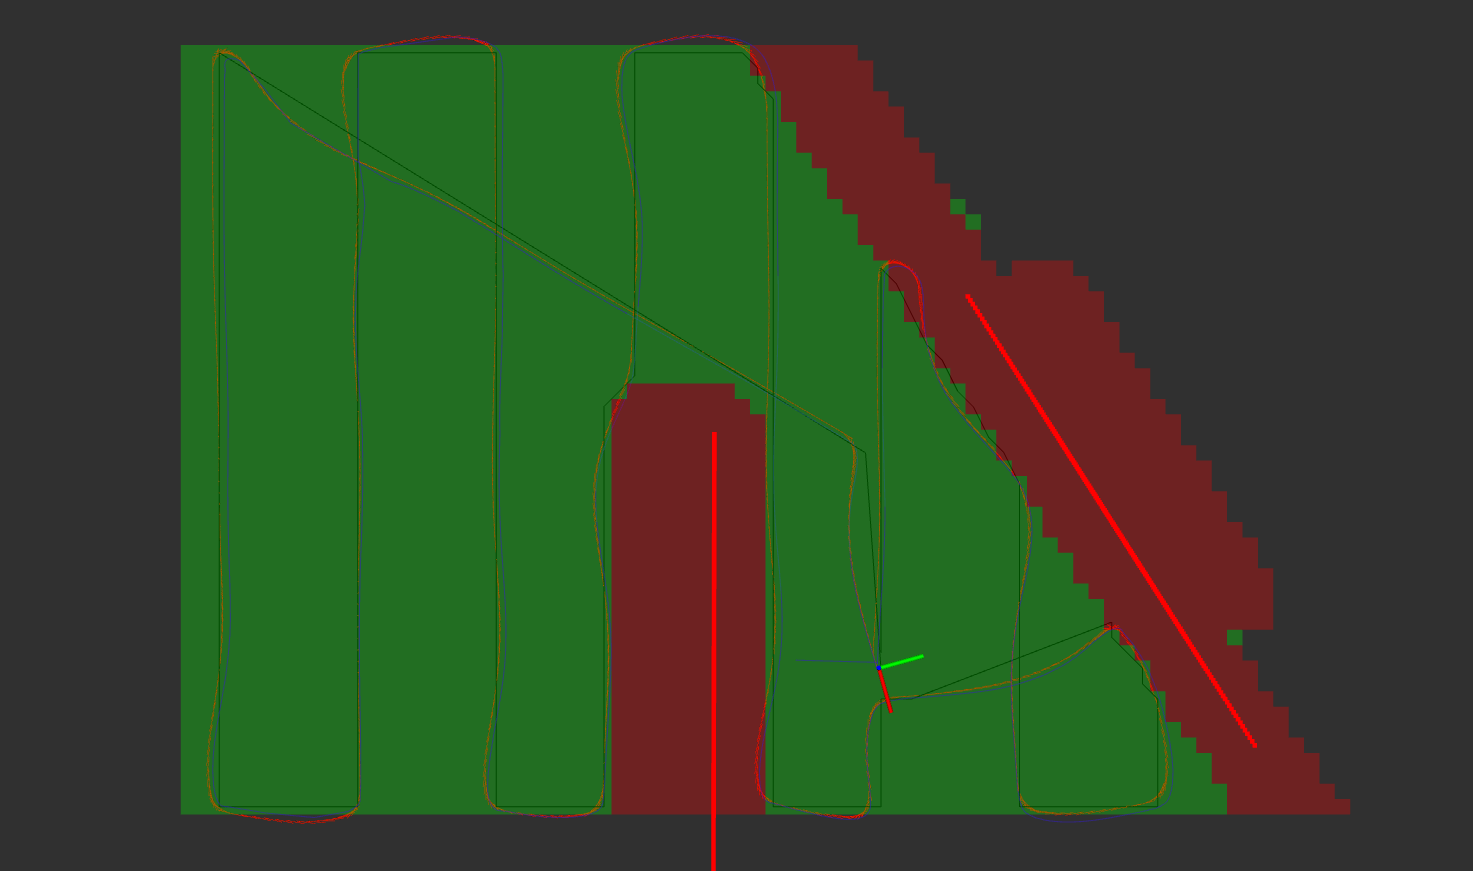
\includegraphics[width=1.0\textwidth,height=0.25\textheight]{fig/simulations/bm1_alg9}
		\caption{}
		\label{fig:bm1_alg_res}
	\end{subfigure}
	\begin{subfigure}[b]{0.5\textwidth}
		\centering
		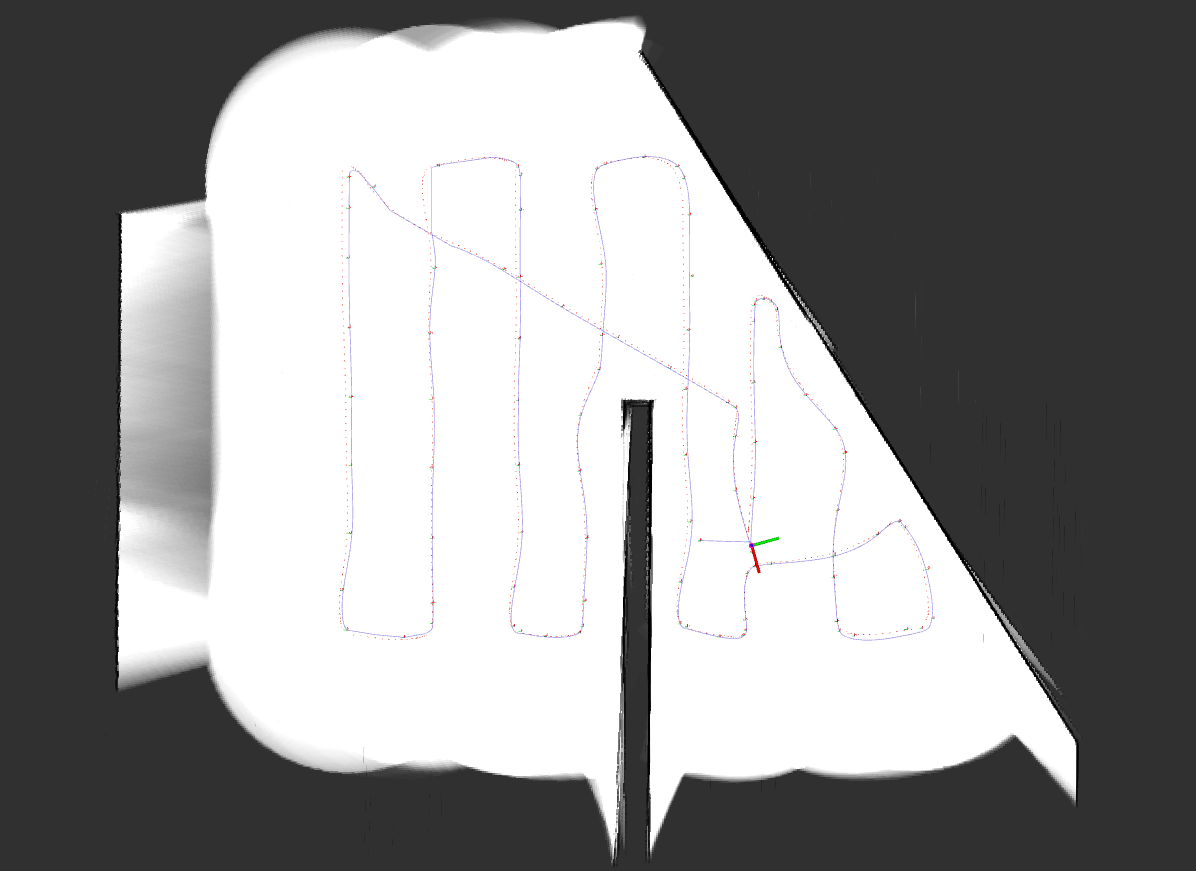
\includegraphics[width=1.0\textwidth,height=0.25\textheight]{fig/simulations/bm1_slam}
		\caption{}
		\label{fig:bm1_slam}
	\end{subfigure}
	}
	\caption[State at the end of the first simulation.]{State at the end of the first simulation. The red and blue curves are the ground truth and estimated trajectories, respectively. (a) Visualization by the system. Covered area is green, inflated obstacles are red, lidar detections are light-red. Black line is the connected waypoints. (b) Map and trajectory by SLAM. The white area of the map represents free space, the black area represents obstacles, and the dark gray area is unknown.}
	\label{fig:bm1_res_res}
\end{figure}

The subfigures of \figref{fig:bm1_res} show how the method reacted during the simulation. (a) In the beginning there is nothing in front of the USV, so the system starts by moving straight ahead. (b) When an obstacle appears in front of the USV, the system knows that there is free space to the right and therefore performs wall following. (c) The bottom of the target region is reached, and the system performs wall following of the virtual wall that is the edge of the target region. (d) A critical point is reached, so the system plans a path to the closest backtracking point. (e) The system reached the backtracking point and intelligently adjusted it a little to the left so that coverage overlap is reduced. Then it reached the bottom of the target region, figured out that the sweeping direction must be switched, and wall followed to the left. When turning back up, there is some coverage overlap because an obstacle blocks the USV from going further left. (f) After reaching the top of the region and coming back down, the system performs a little wall following in order to get to the side of the obstacle. (g) When coming back up the inter-lap spacing is chosen such that there are no uncovered cells left between the current and previous lap, even though some wall following occurred in the middle of the previous lap. (h) The remaining area of the target region is covered. 

% big figure --> decrease margins
\newgeometry{top=2cm,right=1.7in,left=1.7in,bottom=3cm}

\begin{figure}[h!]
    \centering
    \makebox[\linewidth][c]{
	\begin{subfigure}[b]{0.5\textwidth}
		\centering
		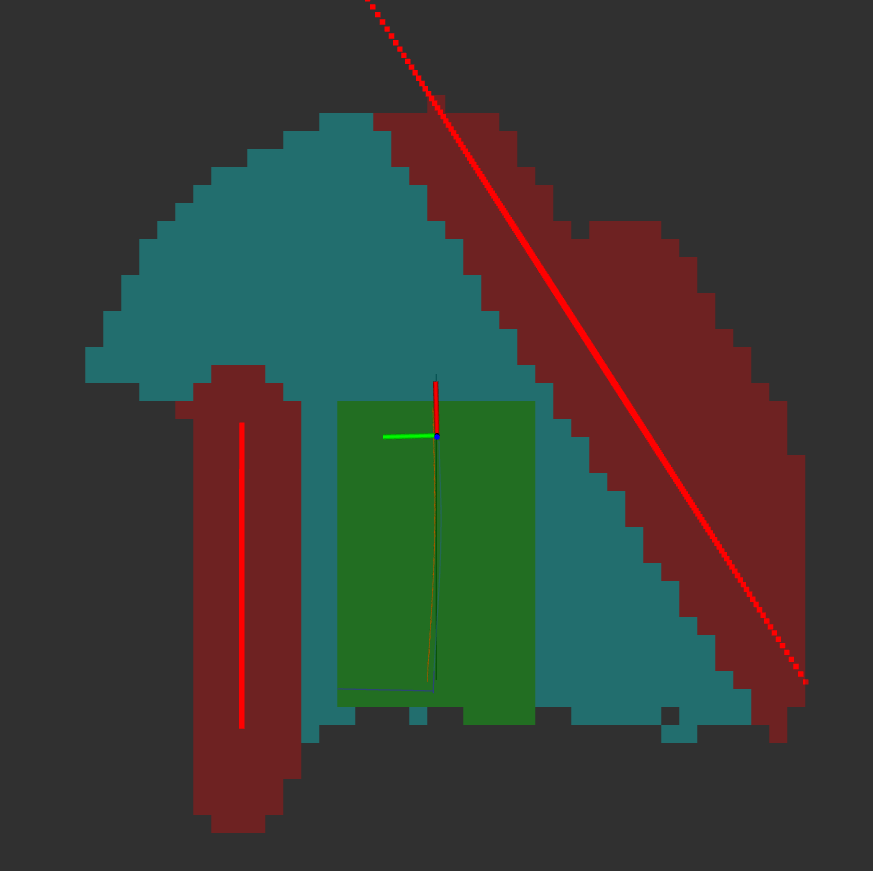
\includegraphics[height=0.20\textheight,width=1\textwidth]{fig/simulations/bm1_alg1_2}
		\caption{}
	\end{subfigure}
	\begin{subfigure}[b]{0.5\textwidth}
		\centering
		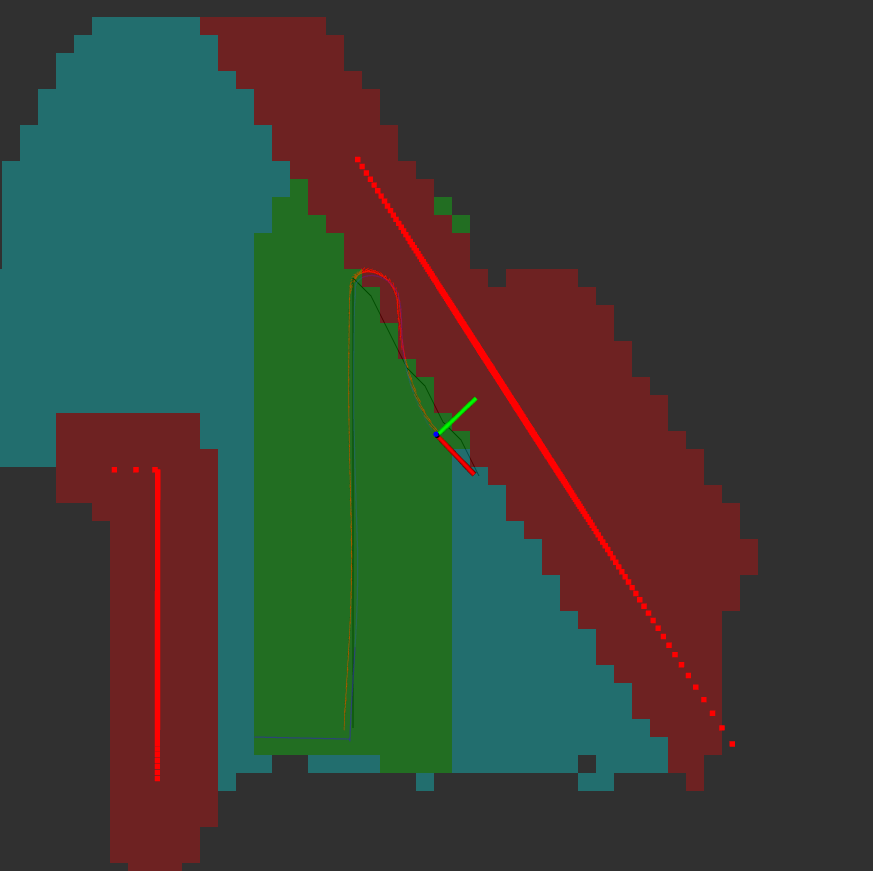
\includegraphics[height=0.20\textheight,width=1\textwidth]{fig/simulations/bm1_alg2_2}
		\caption{}
	\end{subfigure}
	}
	\makebox[\linewidth][c]{
	\begin{subfigure}[b]{0.5\textwidth}
		\centering
		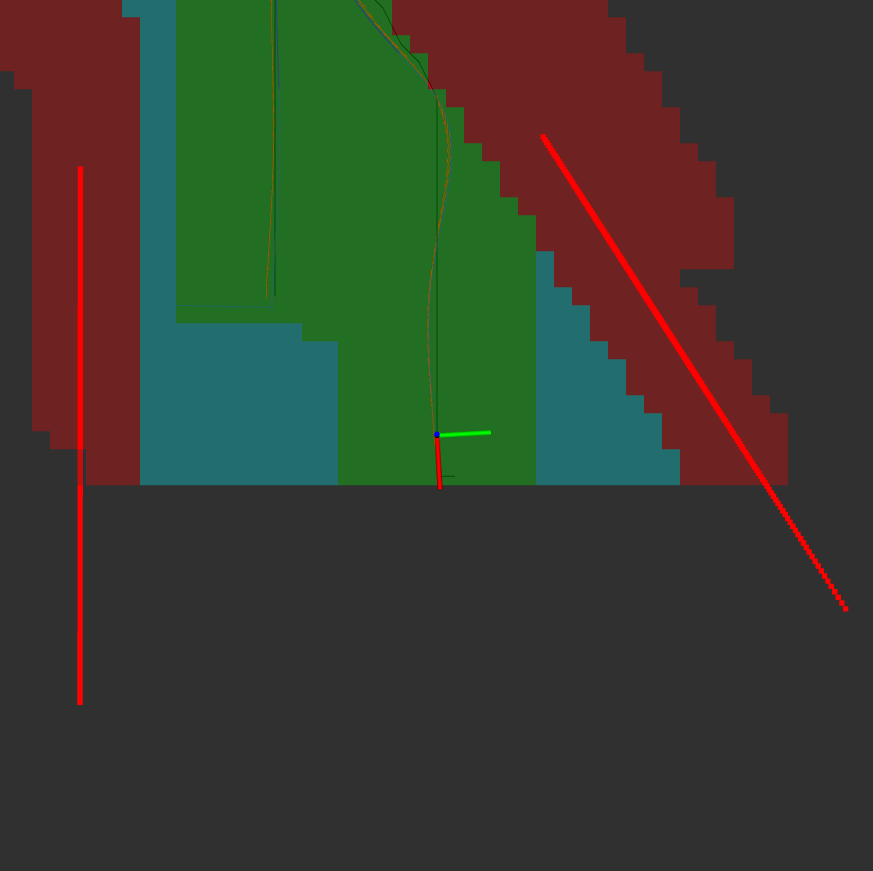
\includegraphics[height=0.20\textheight,width=1\textwidth]{fig/simulations/bm1_alg3_2}
		\caption{}
	\end{subfigure}
	\begin{subfigure}[b]{0.5\textwidth}
		\centering
		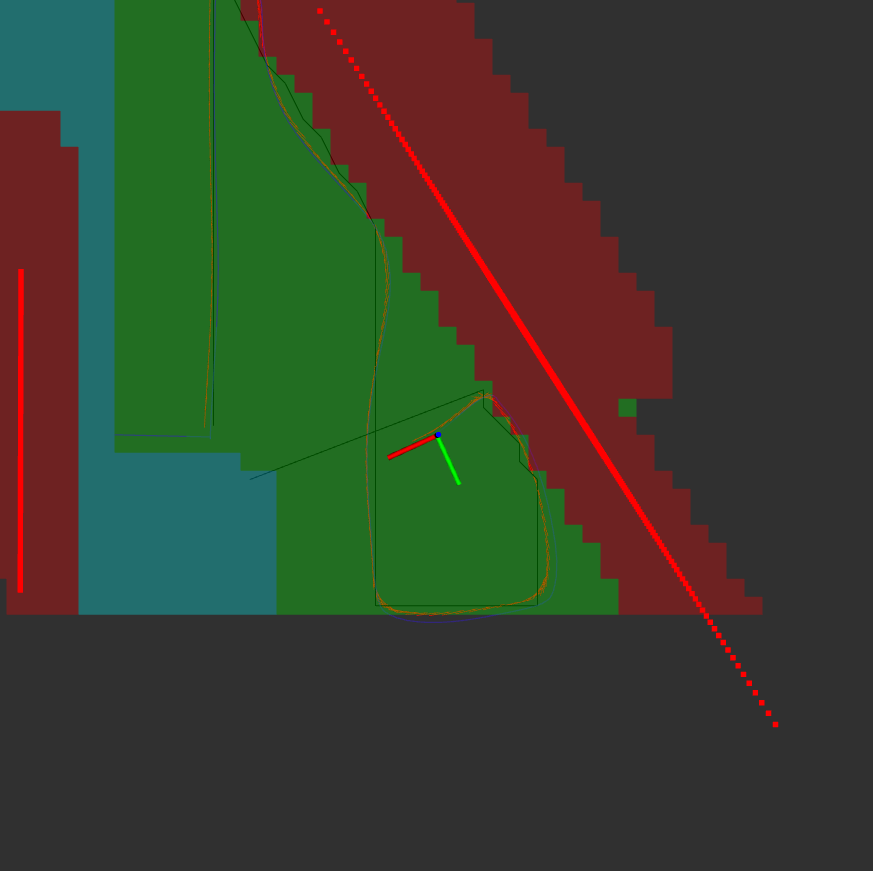
\includegraphics[height=0.20\textheight,width=1\textwidth]{fig/simulations/bm1_alg4_2}
		\caption{}
	\end{subfigure}
	}
	\makebox[\linewidth][c]{
	\begin{subfigure}[b]{0.5\textwidth}
		\centering
		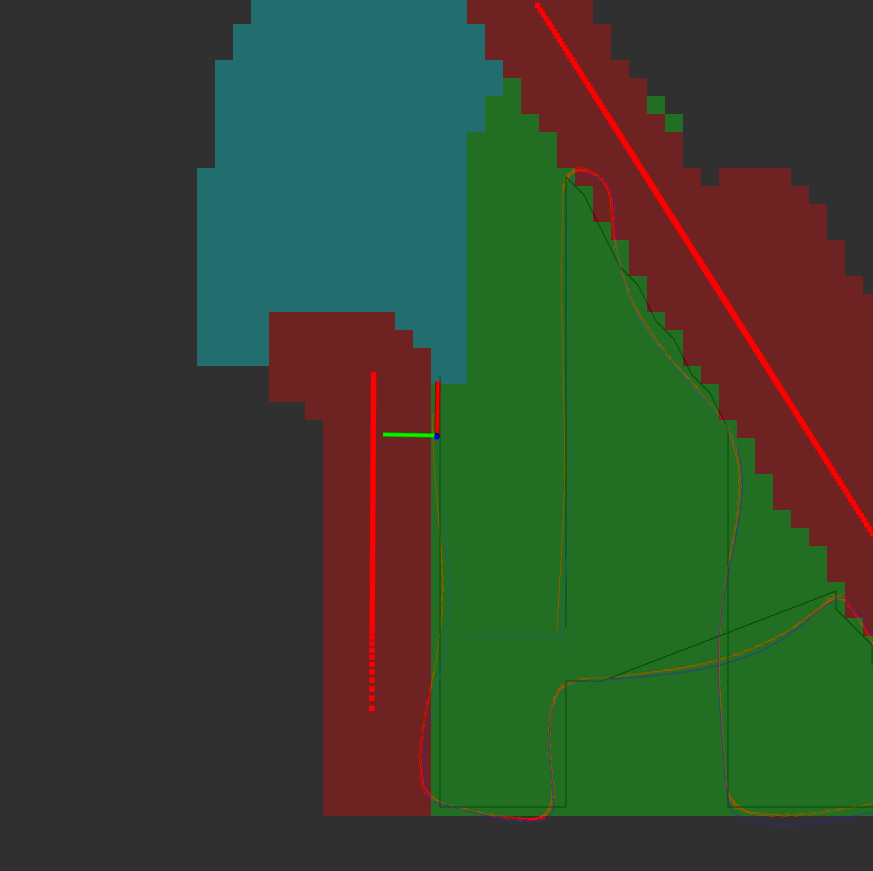
\includegraphics[height=0.20\textheight,width=1\textwidth]{fig/simulations/bm1_alg5_2}
		\caption{}
	\end{subfigure}
	\begin{subfigure}[b]{0.5\textwidth}
		\centering
		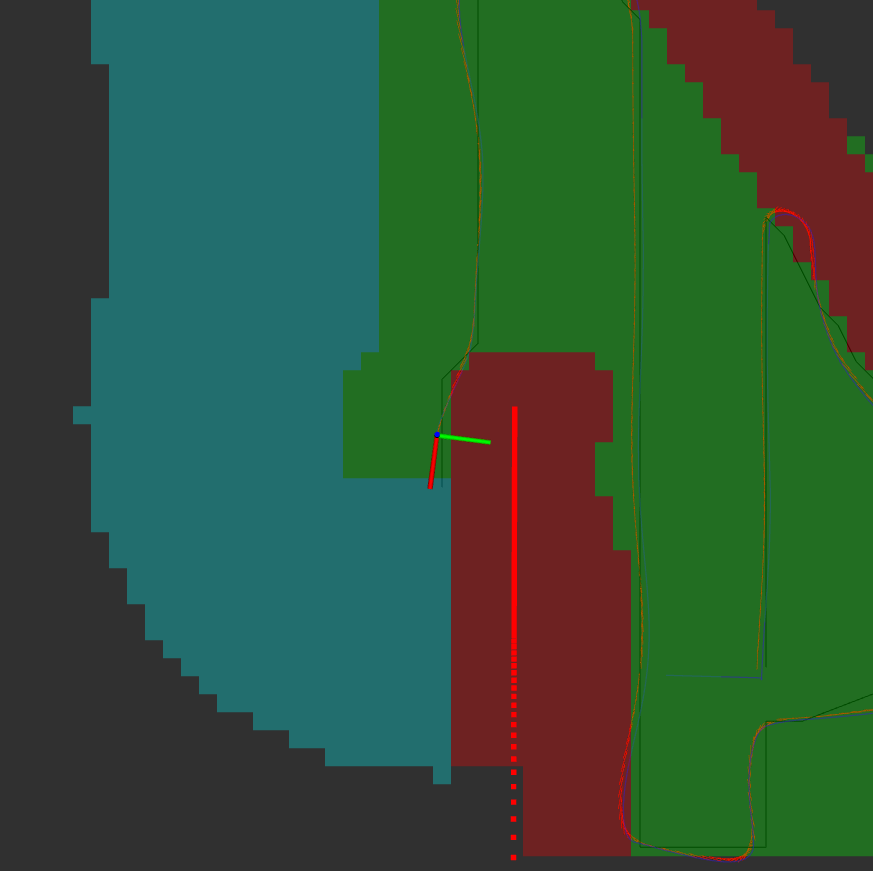
\includegraphics[height=0.20\textheight,width=1\textwidth]{fig/simulations/bm1_alg6_2}
		\caption{}
	\end{subfigure}
	}
	\makebox[\linewidth][c]{
	\begin{subfigure}[b]{0.5\textwidth}
		\centering
		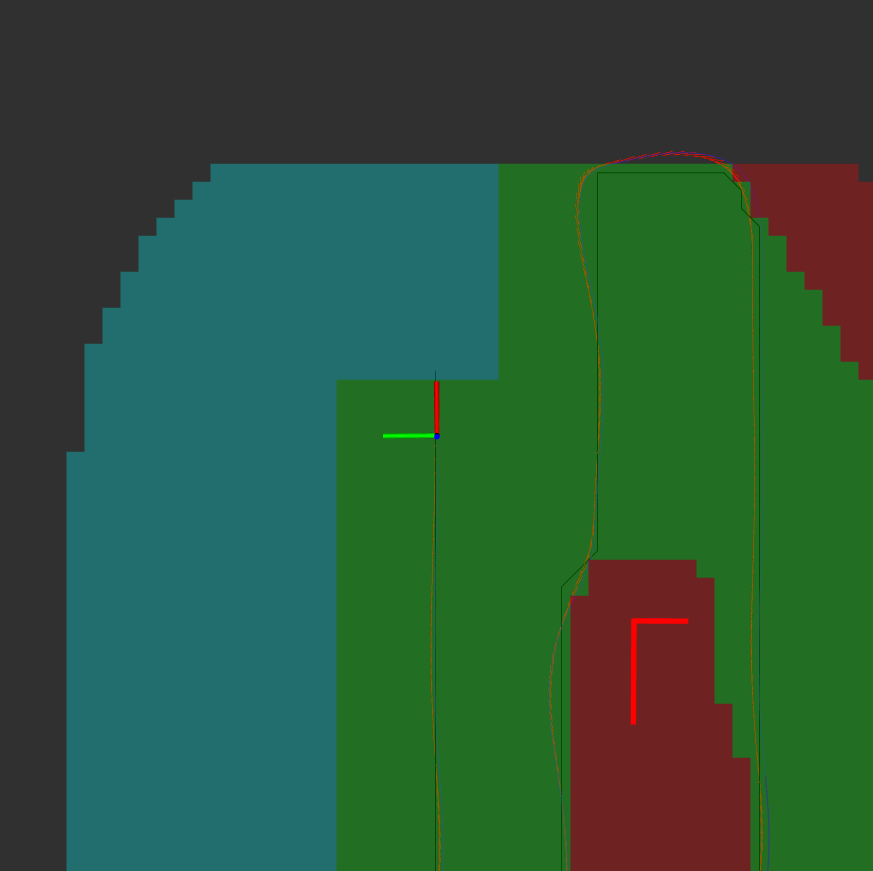
\includegraphics[height=0.20\textheight,width=1\textwidth]{fig/simulations/bm1_alg7_2}
		\caption{}
	\end{subfigure}
	\begin{subfigure}[b]{0.5\textwidth}
		\centering
		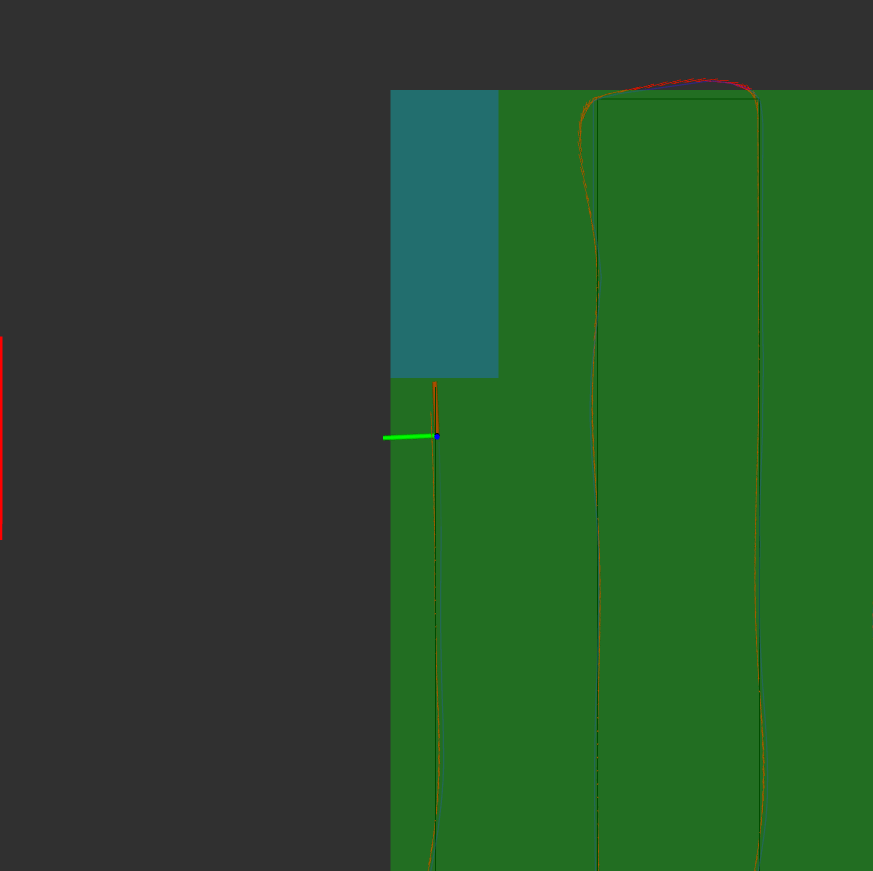
\includegraphics[height=0.20\textheight,width=1\textwidth]{fig/simulations/bm1_alg8_4}
		\caption{}
	\end{subfigure}
	}
    \caption[Visualization of the boustrophedon motions method with constant coverage range at several stages during the simulation.]{Visualization of the boustrophedon motions method with constant coverage range at several stages during the simulation. The red-green-blue axis is the pose of the USV (z-axis positive upwards). Free covered area is represented by green, free uncovered area by blue, and inflated obstacles by red. The light-red dots are the current detection points of the lidar. The black line is the waypoints connected by line segments. The red curve trailing the USV is the ground truth trajectory, while the faint blue curve (often concealed by the red) is the estimated trajectory.}
	\label{fig:bm1_res}
\end{figure}

\FloatBarrier


\subsection{Varying coverage range}

\figref{fig:bm2_sim_env}a shows the target region and surrounding environment of this simulation. \figref{fig:bm2_sim_env}b shows the same region's depth. A simple linearly varying depth seabed which is at its deepest on the left, and at its shallowest on the right. More specifically, the coverage range varies from $\SI{14}{\meter}$ at the far left, to $\SI{4}{\meter}$ at the far right. All parameters of the system are the same as in the previous simulation.

\begin{figure}[h!]
    \centering
	\makebox[\linewidth][c]{
	\begin{subfigure}[b]{0.5\textwidth}
		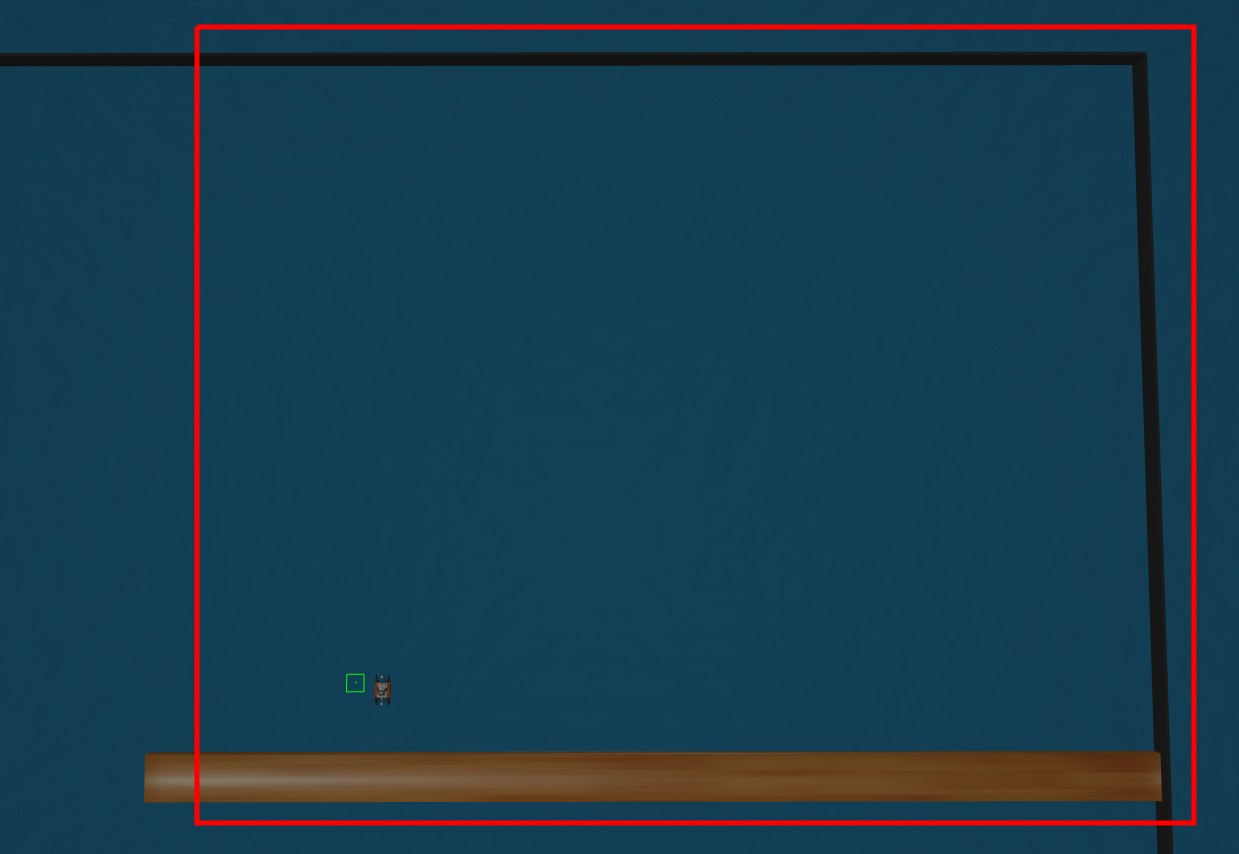
\includegraphics[width=1.0\textwidth]{fig/simulations/target_region_bm_2}
		\caption{}
		\label{fig:bm2_tar_reg}
	\end{subfigure}
	\begin{subfigure}[b]{0.5\textwidth}
		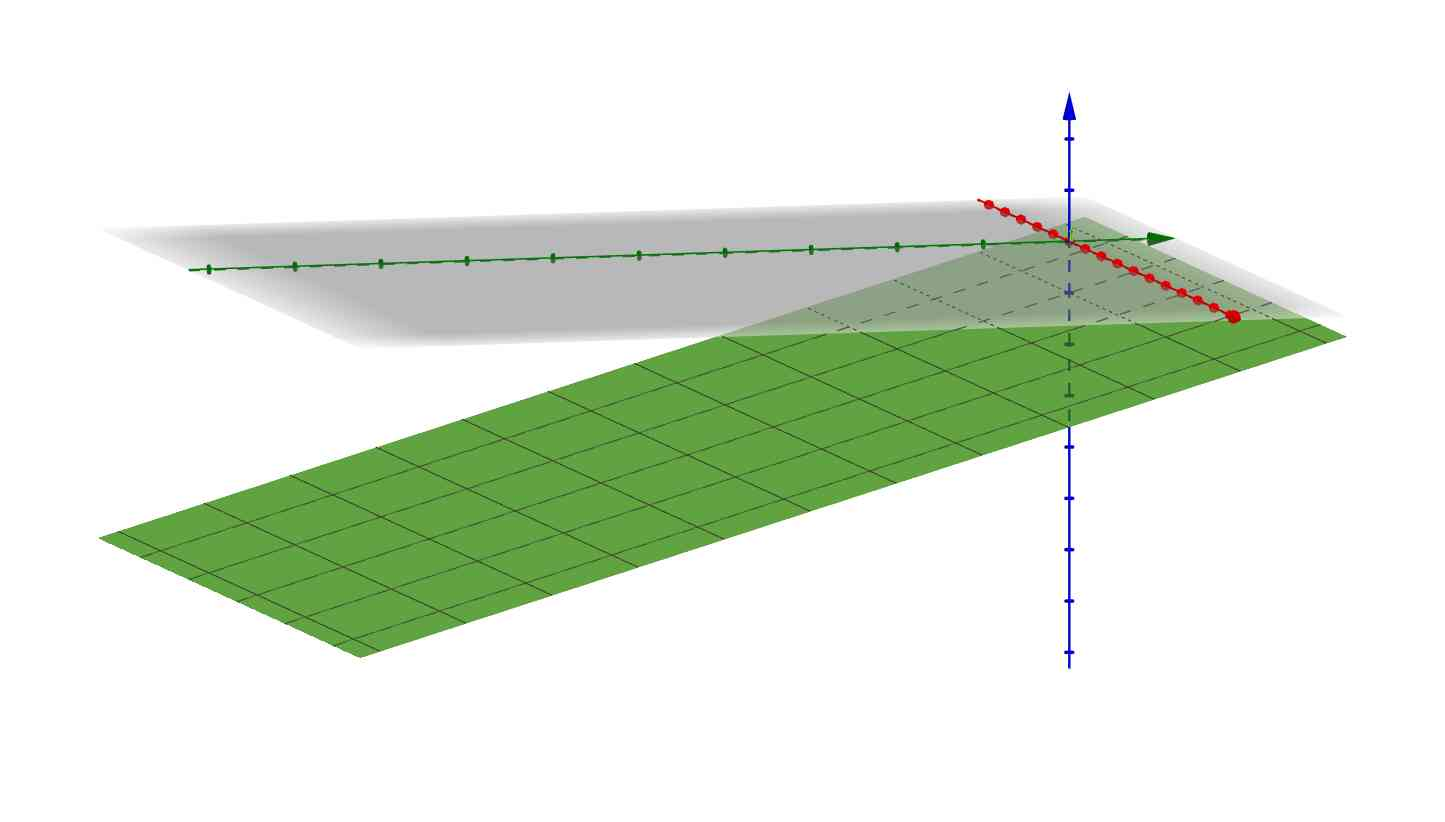
\includegraphics[width=1.0\textwidth]{fig/simulations/bm2_depth.jpg}
		\caption{}
		\label{fig:bm2_depth}
	\end{subfigure}
	}
	\caption[The surrounding environment and target region for the second simulation.]{The second simulation. (a) The surrounding environment and target region. (b) The target region's varying depth seabed.}
	\label{fig:bm2_sim_env}
\end{figure} 

\figref{fig:bm2_alg} shows the result at the end of the simulation, and \figref{fig:bm2_slam} shows the map generated by SLAM at the end of the simulation. \figref{fig:bm2_res} shows the visualization by the system at several stages during the execution. 

\begin{figure}[h!]
    \centering
	\makebox[\linewidth][c]{
	\begin{subfigure}[b]{0.5\textwidth}
		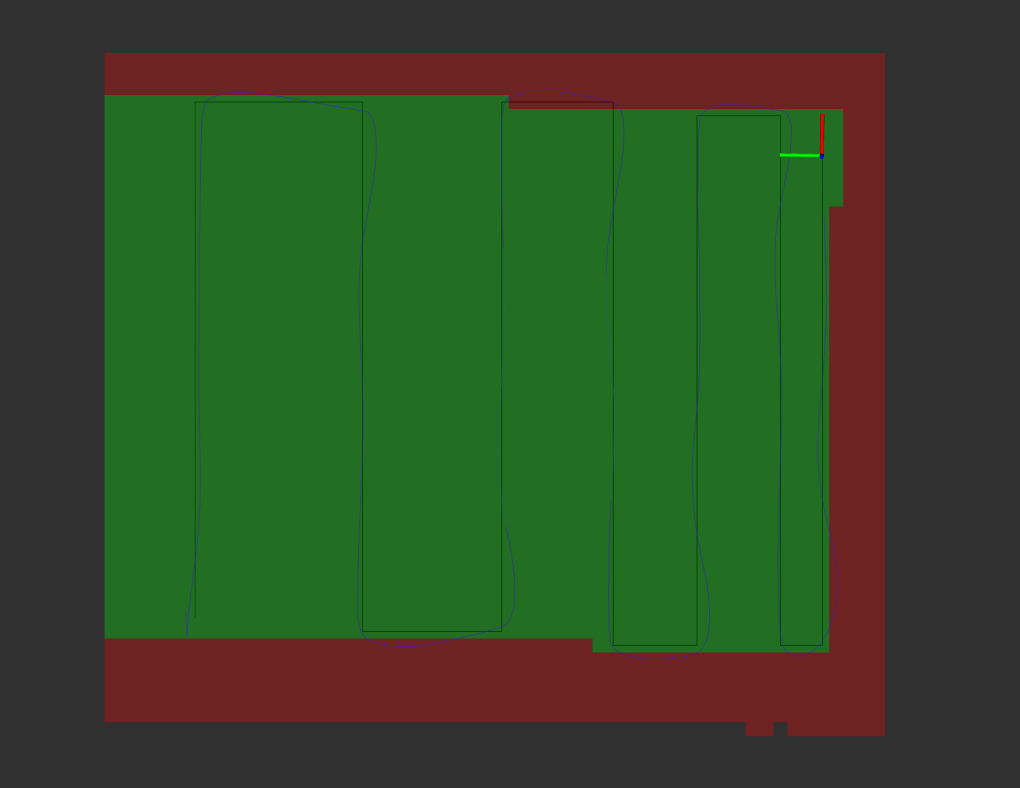
\includegraphics[width=1.0\textwidth,height=0.2\textheight]{fig/simulations/bm2_alg_res}
		\caption{}
		\label{fig:bm2_alg}
	\end{subfigure}
	\begin{subfigure}[b]{0.5\textwidth}
		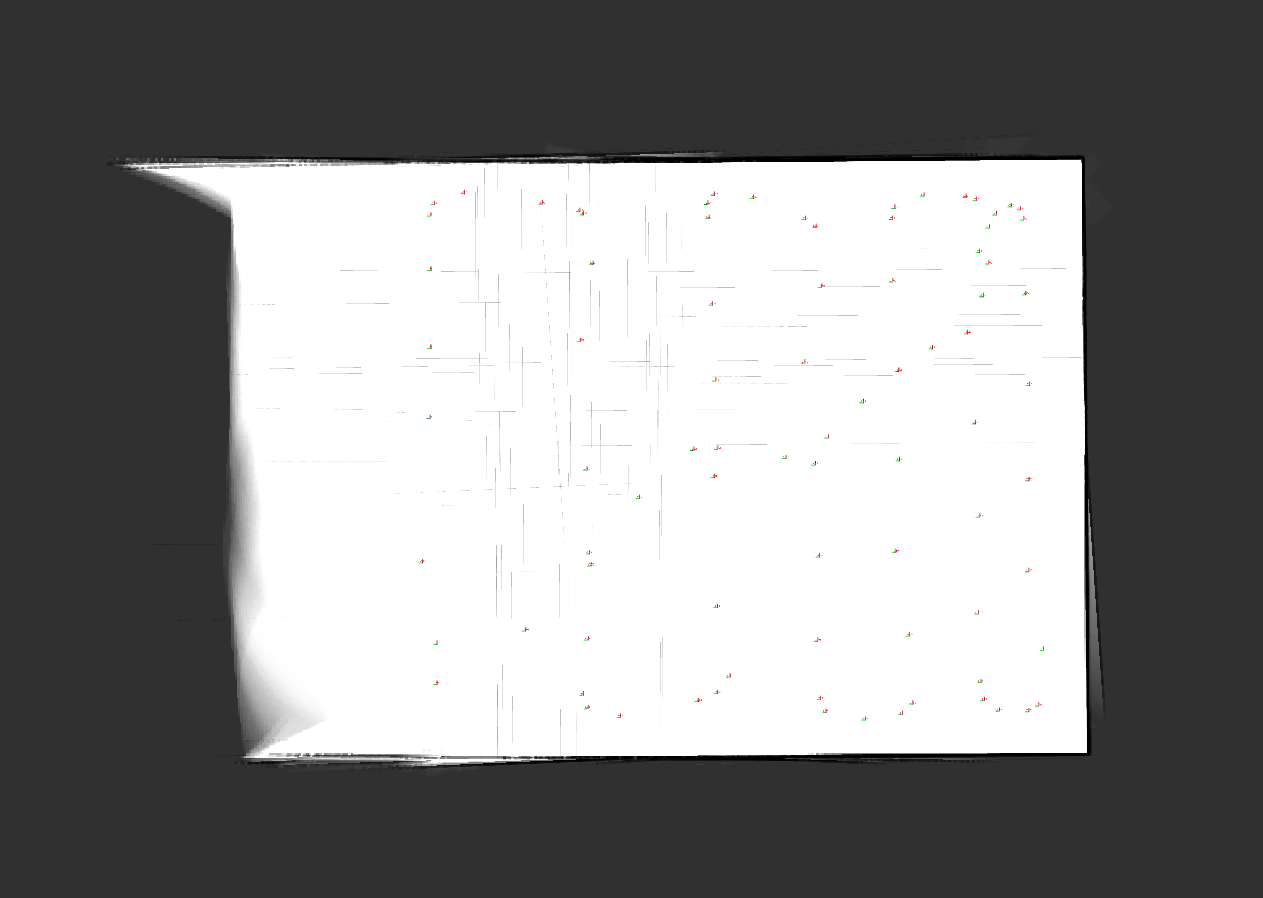
\includegraphics[width=1.0\textwidth,height=0.2\textheight]{fig/simulations/bm2_slam}
		\caption{}
		\label{fig:bm2_slam}
	\end{subfigure}
	}
	\caption[State at the end of the second simulation.]{State at the end of the second simulation. (a) Visualization by the system. Covered area is green and inflated obstacles are red. Black line is the connected waypoints. The blue curve is the estimated trajectory. (b) Map and trajectory by SLAM. The white area of the map represents free space, the black area represents obstacles, and the dark gray area is unknown.}
	\label{fig:bm2_alg_res}
\end{figure}

\restoregeometry 

\newgeometry{top=2.5cm,right=1.7in,left=1.7in,bottom=2.5cm}

\begin{figure}[h!]
    \centering
    \makebox[\linewidth][c]{
	\begin{subfigure}[b]{0.5\textwidth}
		\centering
		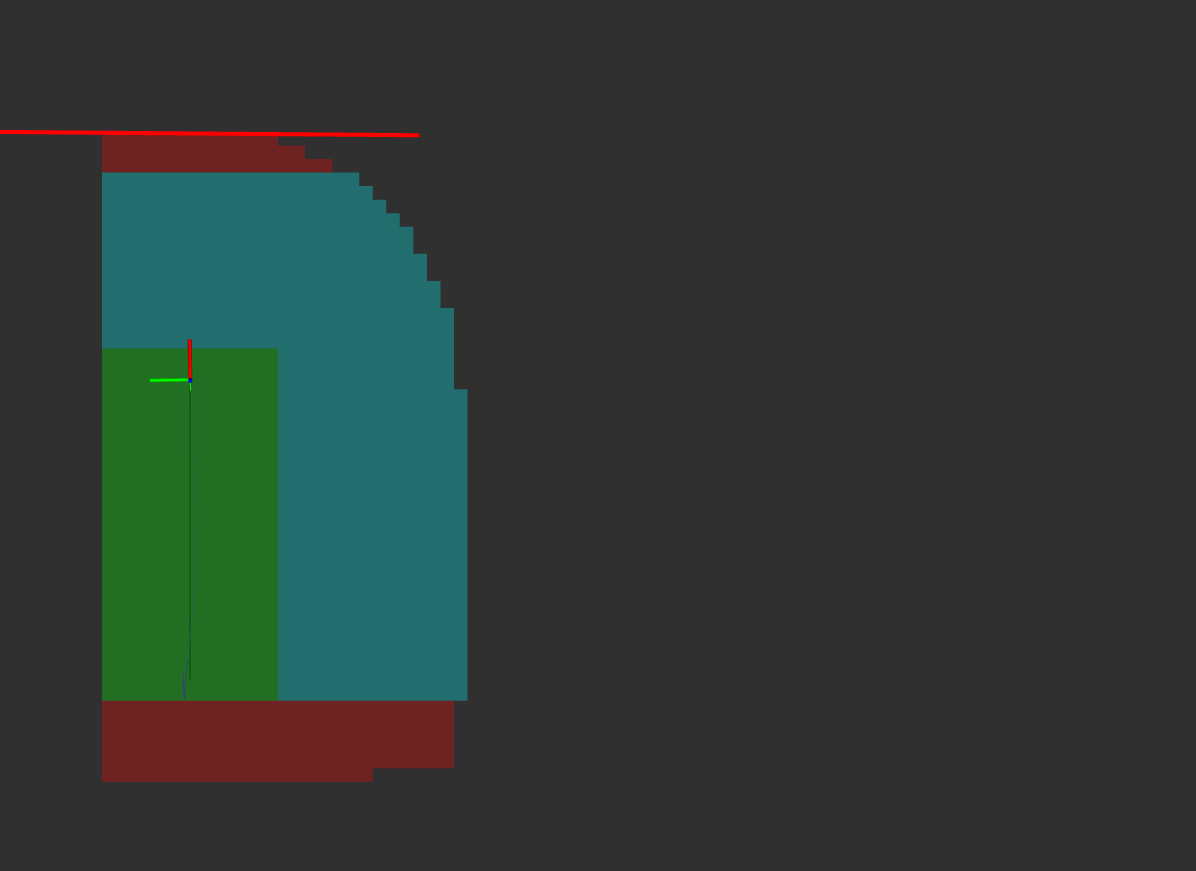
\includegraphics[height=0.20\textheight,width=1\textwidth]{fig/simulations/bm2_alg2}
		\caption{}
	\end{subfigure}
	\begin{subfigure}[b]{0.5\textwidth}
		\centering
		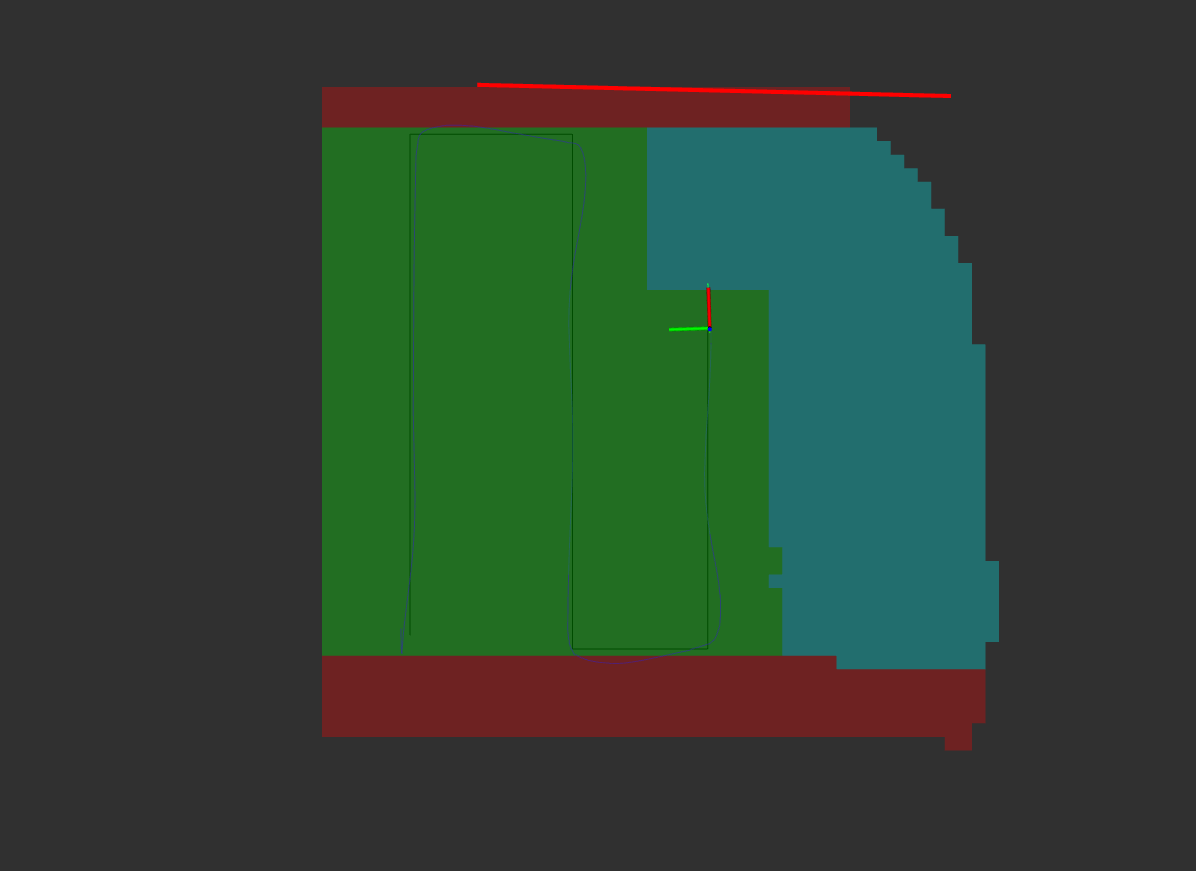
\includegraphics[height=0.20\textheight,width=1\textwidth]{fig/simulations/bm2_alg3}
		\caption{}
	\end{subfigure}
	}
	\makebox[\linewidth][c]{
	\begin{subfigure}[b]{0.5\textwidth}
		\centering
		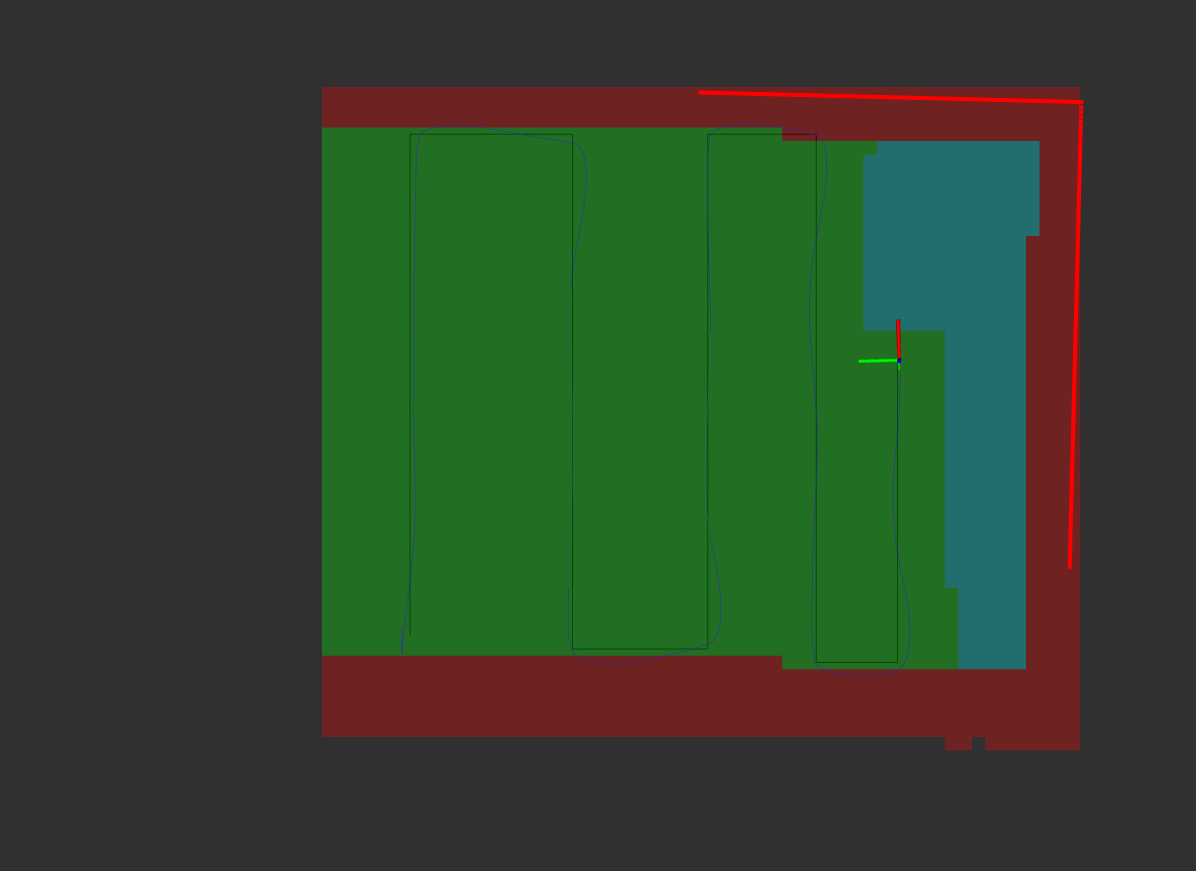
\includegraphics[height=0.20\textheight,width=1\textwidth]{fig/simulations/bm2_alg4}
		\caption{}
	\end{subfigure}
	\begin{subfigure}[b]{0.5\textwidth}
		\centering
		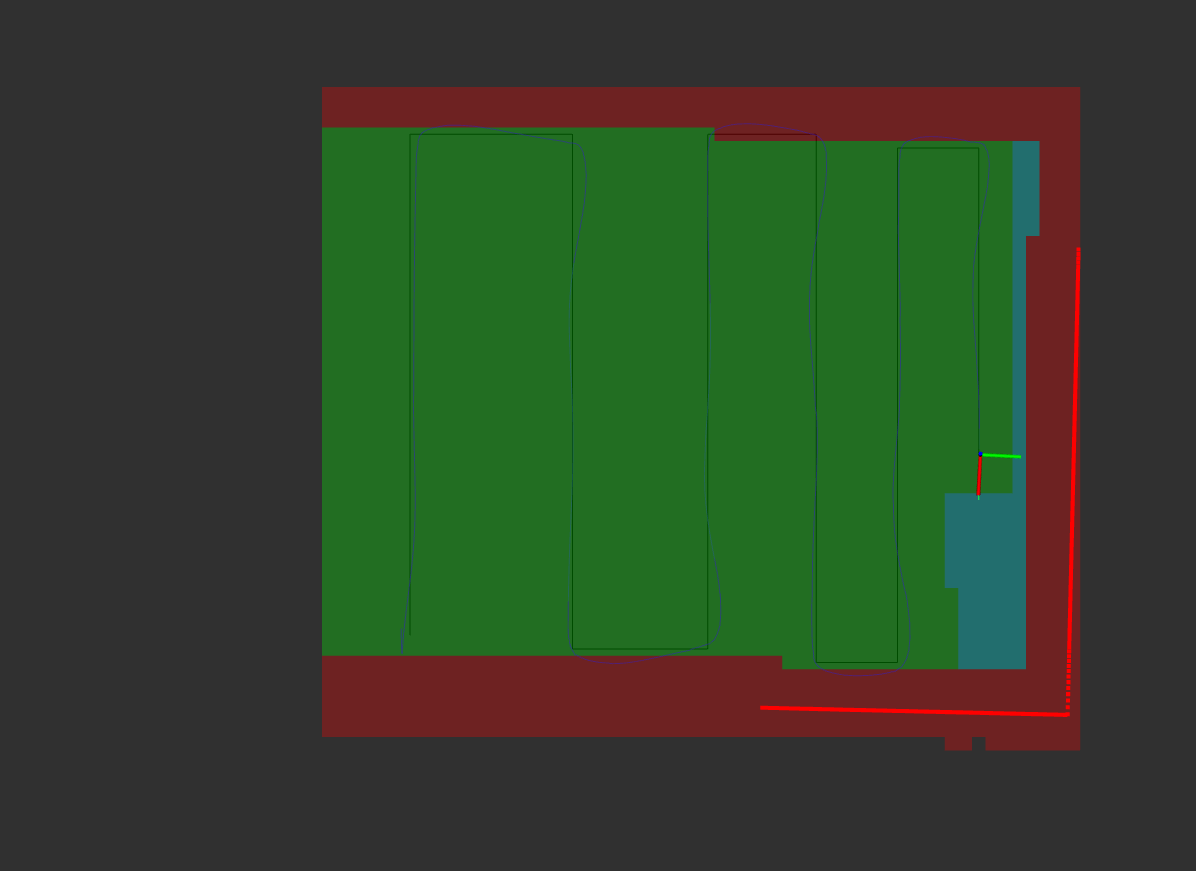
\includegraphics[height=0.20\textheight,width=1\textwidth]{fig/simulations/bm2_alg5}
		\caption{}
	\end{subfigure}
	}
    \caption[Visualization of the boustrophedon motions method with varying coverage range at several stages during the simulation.]{Visualization of the boustrophedon motions method with varying coverage range at several stages during the simulation. The red-green-blue axis is the pose of the USV (z-axis positive upwards). Free covered area is green, free uncovered area is blue, and inflated obstacles are red. The light-red dots are current lidar detections. The black line is the connected waypoints. The blue curve is the estimated trajectory.}
	\label{fig:bm2_res}
\end{figure}




\section{Complete coverage maneuvering with bio-inspired neural network}

The bio-inspired neural network method was tested with the same target region and environment as in the previous simulation, i.e. the region shown in \figref{fig:bm2_tar_reg}. The parameters of the neural network model used in this simulation are $A = 50$, $B = 0.1$, $D = 0.1$, $\mu = 1$, and $E = 100$. The tuning parameter $\lambda$ is set to $\lambda = 0.1$ in order to prioritize areas that do not require a change of direction. The scaling factors $\lambda_i$ have all been set to $\lambda_i = 1$. The set of neighboring neurons is restricted by $r_0 = \sqrt{3}r_c$, meaning only the 6 surrounding circles in the partition are considered neighbors. The circles in the partition all have a radius of $r_c = \SI{5}{\meter}$. The rest of the parameters of the system are the same as in the first simulation described in Section \ref{sec:sim1}.

\figref{fig:binn_res} shows the visualization by the system at several stages during the execution, and \figref{fig:binn_slam} shows the map generated by SLAM at the end of the simulation. In \figref{fig:binn_res}, the next target cell is always the cell associated with the neuron that has the highest neural activity, but with a slight preference for going straight forward.



\begin{figure}[h!]
    \centering
    \makebox[\linewidth][c]{
	\begin{subfigure}[b]{0.5\textwidth}
		\centering
		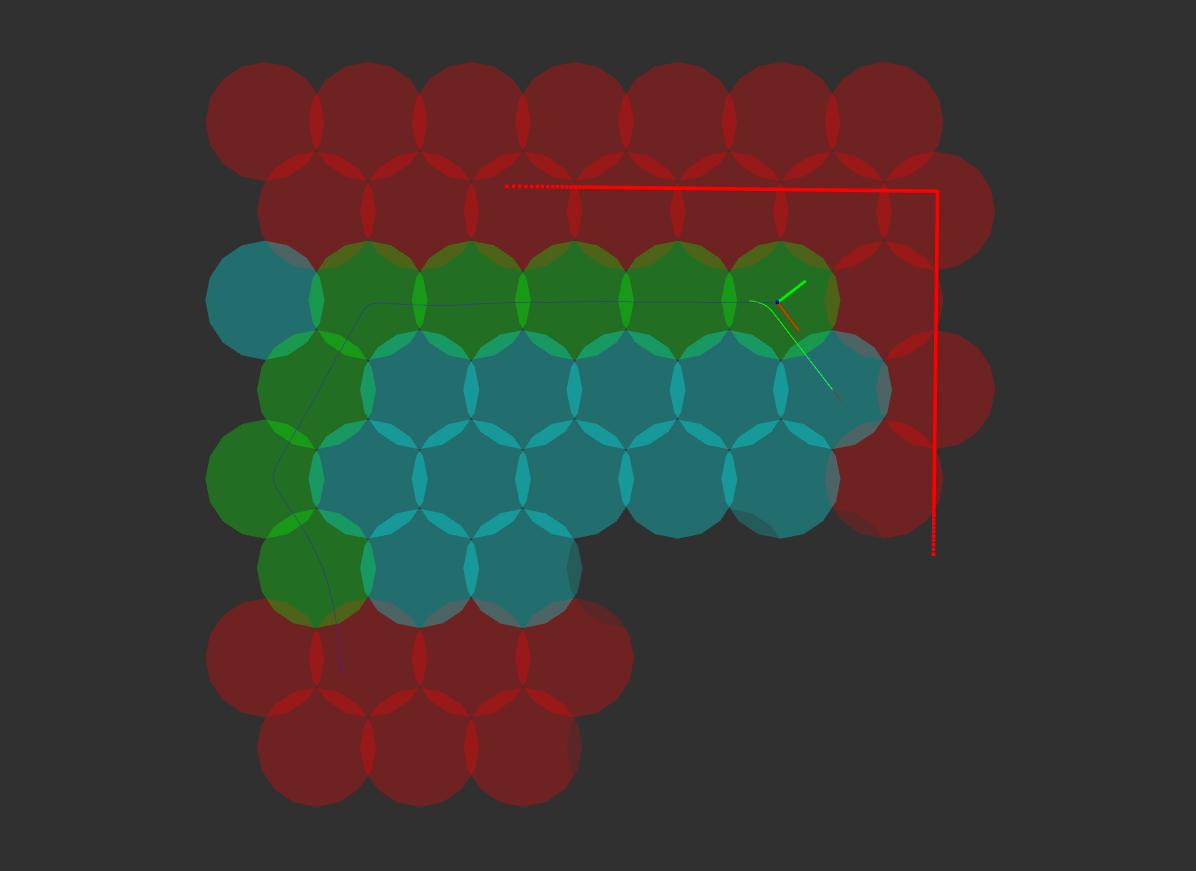
\includegraphics[height=0.20\textheight,width=1\textwidth]{fig/simulations/binn_alg1}
		\caption{}
	\end{subfigure}
	\begin{subfigure}[b]{0.5\textwidth}
		\centering
		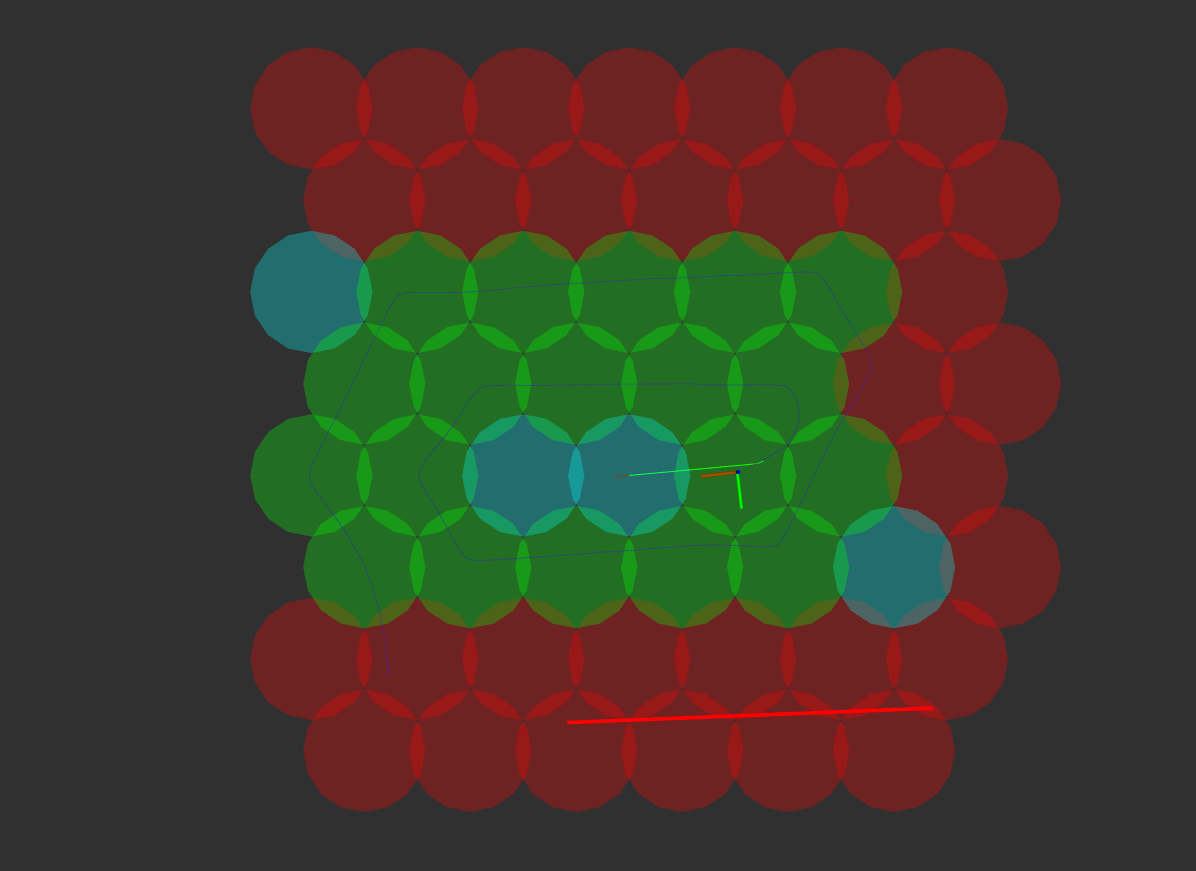
\includegraphics[height=0.20\textheight,width=1\textwidth]{fig/simulations/binn_alg3}
		\caption{}
	\end{subfigure}
	}
	\makebox[\linewidth][c]{
	\begin{subfigure}[b]{0.5\textwidth}
		\centering
		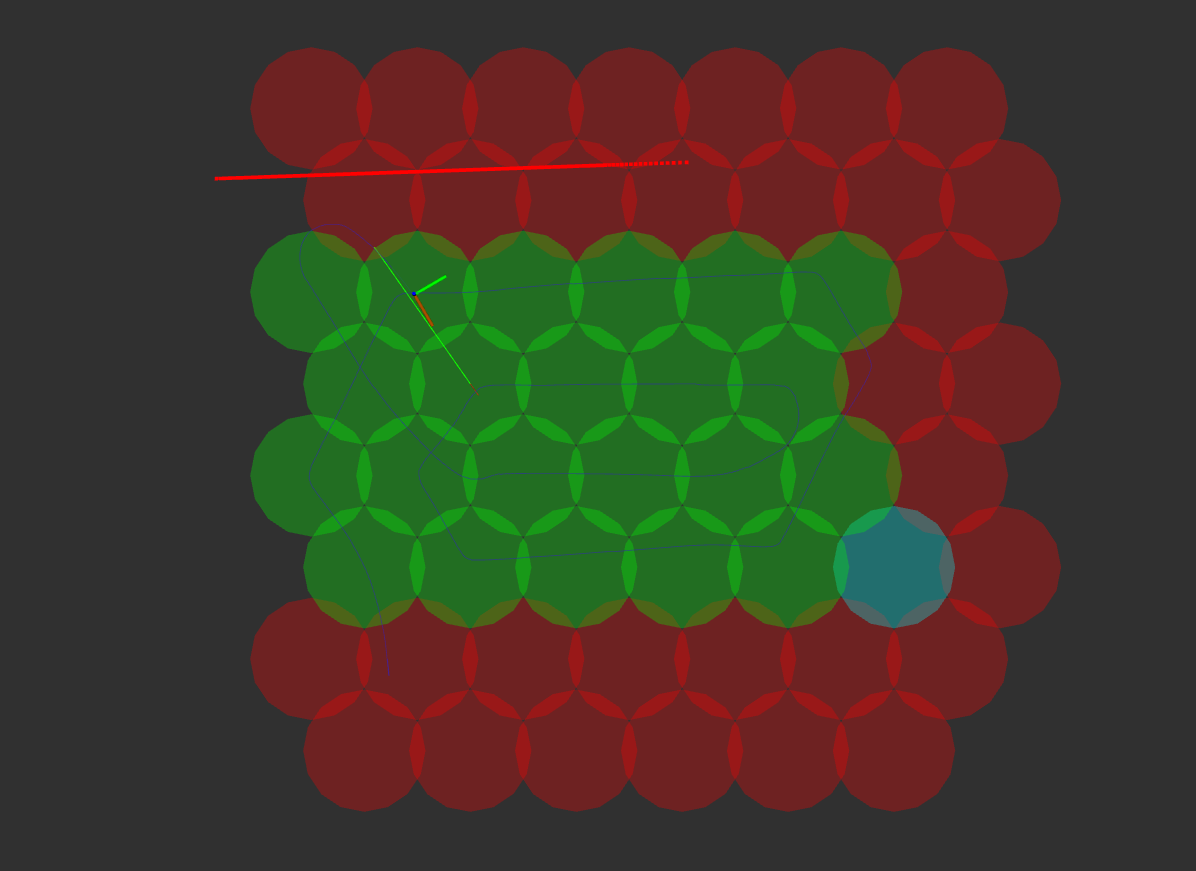
\includegraphics[height=0.20\textheight,width=1\textwidth]{fig/simulations/binn_alg4}
		\caption{}
	\end{subfigure}
	\begin{subfigure}[b]{0.5\textwidth}
		\centering
		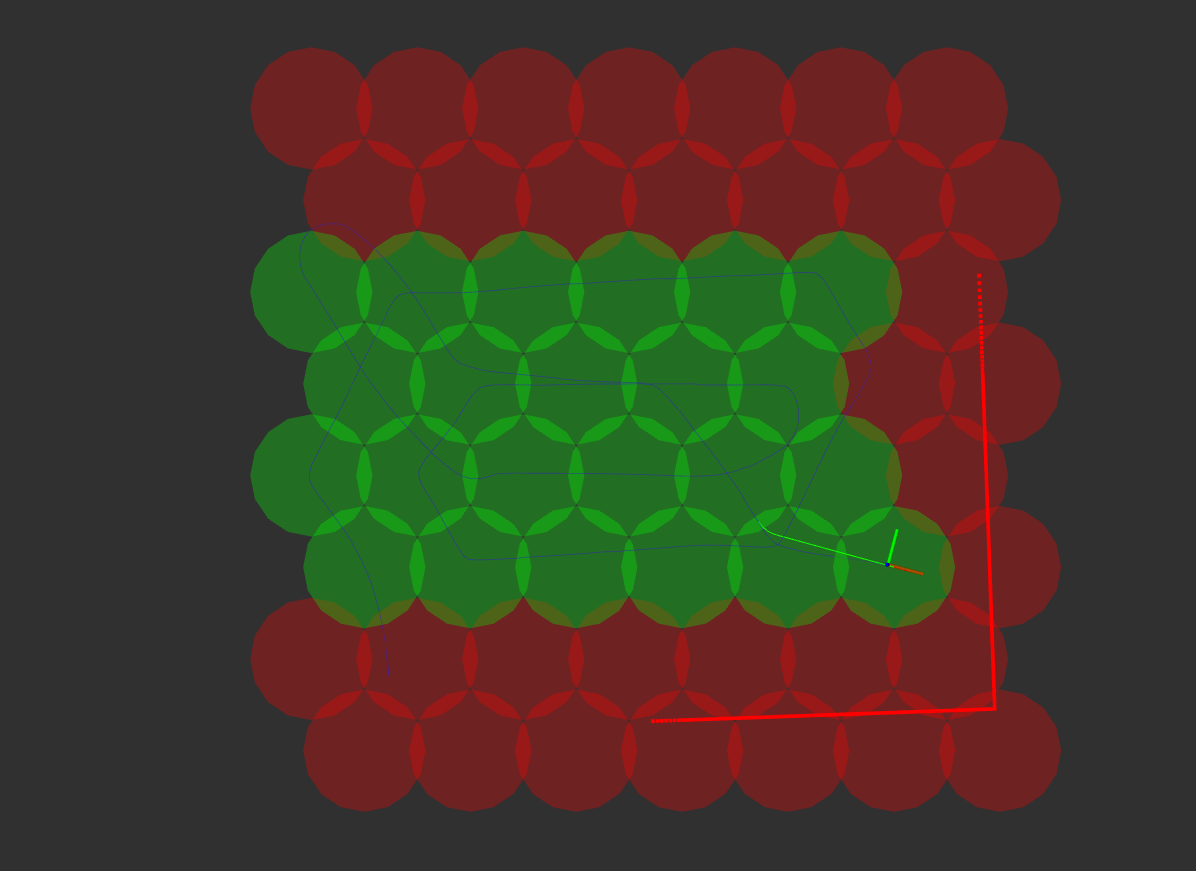
\includegraphics[height=0.20\textheight,width=1\textwidth]{fig/simulations/binn_alg5}
		\caption{}
	\end{subfigure}
	}
	\caption[Visualization of the bio-inspired neural network method at several stages during the simulation.]{Visualization of the bio-inspired neural network method at several stages during the simulation. The red-green-blue axis is the pose of the USV (z-axis positive upwards). Free covered area is green, free uncovered area is blue, and inflated obstacles are red. The light-red dots are current lidar detections. The blue curve is the estimated trajectory. The green curve is the currently followed simple Dubins path.}
	\label{fig:binn_res}
\end{figure}

\begin{figure}[h!]
	\centering
	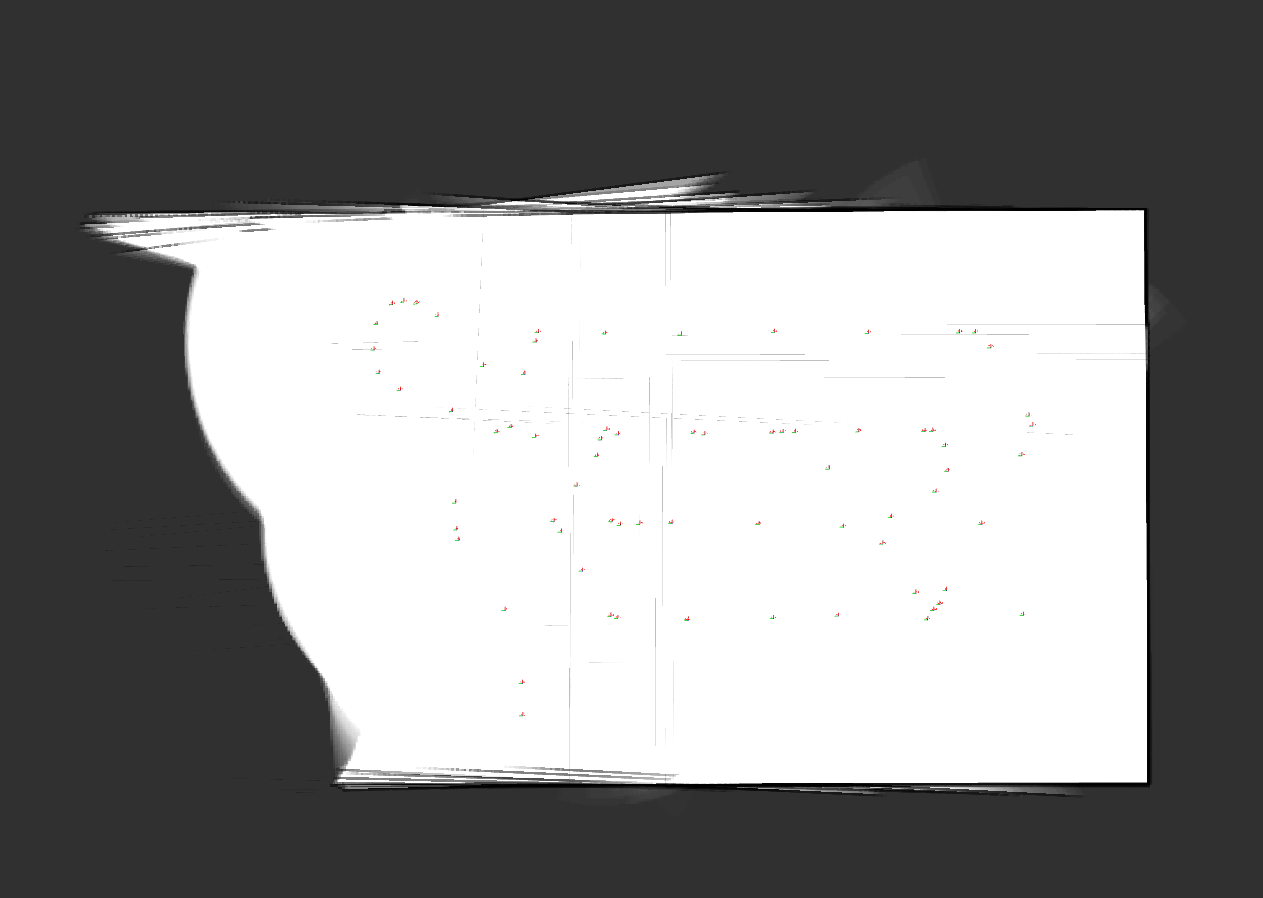
\includegraphics[width=0.7\textwidth]{fig/simulations/binn_slam}
	\caption[Map by SLAM at the end of the third simulation.]{Map by SLAM at the end of the third simulation. The white area of the map represents free space, the black area represents obstacles, and the dark gray area is unknown.}
	\label{fig:binn_slam}
\end{figure}

\restoregeometry 


\section{Discussion}

\subsection{Sensor fusion and SLAM}

The SLAM map generated in \figref{fig:sim_sensor_fusion} quite accurately depicts the simulated environment. The walls are straight, there is a clear transition between obstacles and free space, and the proportions look very reasonable. Because of the lidar's restricted range of only 25 m, the SLAM system is never able to see across the middle, and thus this area remains uncertain. In the top left corner, there is an opening without any walls. Even though the USV traveled across this area, the area still remains uncertain in the map. It could be reasoned that everything within the lidar's range should be considered free space when there are no detections. However, since a lidar's range varies depending on the reflectivity of the material and lighting conditions, care must be taken when assuming free space in the case of no detections. Cartographer has a parameter allowing to set the distance for assumed free space. In this case, the purpose was to create an accurate map, so there was no reason to assume free space.

\figref{fig:bm1_slam} shows the SLAM map, estimated trajectory, and ground truth trajectory for the first simulation. The SLAM map accurately depicts the target region in \figref{fig:target_region_bm_1}. Looking closely at the map, there have been some small errors, as evident by the short strips of duplicated walls on the right-most inclined wall. This is caused by the SLAM system thinking for a short time that it has a different pose than it really has, and then mapping the environment at the wrong place. In a carefully tuned system, such errors should rarely be seen. There are also some inaccuracies in the mapping of the jetty in the middle of the map. Overall, however, the mapping looks good. The estimated trajectory also approximates the ground truth well. It can be seen to drift a little at times, but it always corrects itself.

The results of the second and third simulations in \figref{fig:bm2_slam} and \figref{fig:binn_slam} show many of the same properties. These maps both depict the environment of \figref{fig:bm2_tar_reg}. It should be noted, however, that the bio-inspired neural network method used to create the map in \figref{fig:binn_slam} results in more errors in the map. This is likely because this method causes the USV to turn more, which is more difficult for accurate pose estimation. In particular, turns performed when the lidar detects nothing, i.e. when the USV is far from obstacles, prevents corrections to pose estimations by loop closure. The map can only be corrected with loop closures after the lidar starts detecting obstacles again. If no distinct features are then detected, the accumulated errors in localization might be too big and difficult to correct for. 

This last argument highlights another very important issue for this particular application. Namely, that the range of the lidar is very short compared to the size of the workspace. This means the lidar scans are often empty or consist of only a single line-segment of detection points representing the closest wall or jetty. Cartographer is mainly a lidar-based SLAM method, and relies heavily on these lidar scans. The data from the lidar, however, is by itself not nearly enough information to perform SLAM. As a result, the sensor fusion and SLAM system is very dependent on GNSS, even when close to obstacles. 


\subsection{CCPP with boustrophedon motions}


The first simulation is summarized in \figref{fig:bm1_res_res}. \figref{fig:bm1_alg_res} shows that complete coverage is achieved, and upon completion the USV travels back to the starting point and stops there. This is also a great example of how the line-of-sight smoothing of A* paths works as intended. The subfigures of \figref{fig:bm1_res} also verify that the many autonomous subfunctions of the implemented system work as intended in a simulated environment. The localization and map in \figref{fig:bm1_slam} provided by the sensor fusion and SLAM subsystem has also proved to be good enough for the algorithms in the rest of the system to function properly and achieve complete coverage.

The second simulation, in \figref{fig:bm2_alg} and \figref{fig:bm2_res}, shows how the method performed with a simple linearly varying sea depth. The seabed shown in \figref{fig:bm2_depth} is overly simplistic, but the simulation nonetheless showcases the method's ability to react to the varying coverage range of the MBES. 
\figref{fig:bm2_res} shows the coverage range shrinking as the USV moves farther to the right and towards shallower waters. As expected, the inter-lap spacing shrinks to accommodate the smaller coverage range while still avoiding overlapping coverage.

Note that the second simulation shows a very idealistic scenario, where the coverage range is constant along the entire length of one lap. Realistically, even with the best possible sweeping direction, there will be some difference between the shallowest and deepest point in one lap, which will necessarily result in some overlapping coverage. Since the implemented method simply chooses the sweeping direction as the heading angle the system starts with, the choice of sweeping direction is left entirely in the hands of the operator. Leaving this important part of the survey to chance, or to depend on the operator's prior knowledge of the area, is a weakness of the system. A possible extension is therefore to incorporate the ideas of \citet{galceran2012efficient} for choosing the best sweeping direction, although it would have to be done online without any prior knowledge. As suggested in the same paper, a further improvement would be segmentation of the target region into several smaller similar-depth target regions. This would also have to be done online. Developing online algorithms for these two extensions would be a great step forward in the field of autonomous seabed mapping, and would result in a system that incorporates many of the best practices of hydrographic surveying.

\subsection{CCPP with bio-inspired neural network}

The result of running the third simulation with the bio-inspired neural network is shown in \figref{fig:binn_res}. The neural network is set up to always target the neighboring circle with the highest neural activity, but with a preference for reducing turns. As seen in subfigures (a) and (b), this tends to create spiraling patterns. Once the spiral pattern is complete, the remaining uncovered circles are the only cells with high neural activity. Consequently, the system is attracted to these last remaining uncovered cells, as seen in (c) and (d), and achieves complete coverage.

This method tends to create more turns than the boustrophedon motions method, even though the target cell is chosen with a preference for less turning. In the end, this preference actually causes more turns in total. The method ends up always delaying turns to the last possible moment, which is generally not an intelligent way to cover an area with the circular partition used here. Turning reduces not only the accuracy of SLAM as discussed above, but more importantly it reduces the quality of the bathymetric data acquired by the MBES. This is because during turning the accuracy of pose estimation is reduced, which introduces errors in the mapping of the seabed. More turns also increase the duration and fuel consumption of the survey. 

It should be noted that some other works in the literature have achieved somewhat better results with almost the same method (e.g. \citet{Scibilia2012} and \citet{luo2008bioinspired}), and it is likely because of different tuning parameters resulting in a more intelligent path. The performance of the method might see a slight improvement by altering the behavior of the neural network and the choice of the target neuron. For instance by modifying equation \eqref{eq:binn_pos} or choosing the tuning parameter $\lambda_i$ wisely. \citet{Scibilia2012} states for instance that $\lambda_i$ is used to prioritize areas closer to the initial AUV position. The results of \citet{luo2008bioinspired} show paths that look very much like boustrophedon motions. However, they use a square cell partition which, based on these results, might be better suited.

The partition used for this method is not able to adapt to a varying coverage range. Instead, the size of the circular cells must be determined based on the shallowest point in the target region, i.e. the point which results in the minimum coverage range. Doing this ensures complete coverage, but may result in a lot of overlapping coverage if the depth varies a lot. A possible solution to this would be to repartition the target region with another cell size when the depth varies more than some threshold. Alternatively, the target region could be divided into several similar-depth subregions, each with a different cell size depending on the shallowest point within the subregion.

Another drawback of the circular cell partitioning is that the cell size determined by the water depth, also determines how accurately obstacles are represented. In this simulation, the cells have a radius of $r_c = \SI{5.0}{\meter}$ in order to represent the coverage range. This means that an area of free space up to $\SI{20.0}{\meter}$ wide may be considered an obstacle with an unfortunate placement of the circles. By comparing the resulting coverage of \figref{fig:bm2_alg} and \figref{fig:binn_res}d, it is clear that the circular partition does a worse job of representing obstacles. The square cell partitioning avoids these issues by separating the coverage range from the cell size, and allowing multiple cells to be marked as covered together. An obvious further development of the bio-inspired neural network CCPP method would therefore be to incorporate the square cell partitioning instead.

\subsection{Path following}

\figref{fig:bm1_alg_res} shows that the ground truth trajectory (red line) manages to track the waypoints (black line) well. Keep in mind that the path that is actually followed is not the black line connecting the waypoints, but a simple Dubins path generated from the USV's pose to the newest waypoint. This means that the overshoot that appears around sharp corners such as in \figref{fig:bm1_res}b is to be expected, because the generated simple Dubins path accounts for the turning radius. This also means that the planned simple Dubins path often goes outside the green and blue region classified as free space in the partition, and into the red region classified as inflated obstacles. As long as obstacles are inflated with a radius greater than the maximum USV footprint plus the turning radius, i.e. $r_i > r_{max} + \rho$, the USV will avoid collision. However, this should be done more intelligently, because the increased obstacle inflation radius means that the coverage of the seabed close to or beneath obstacles is reduced. Consider the possibility of inflating obstacles in two steps instead, first to incorporate the USV footprint and then secondly to incorporate the turning radius. This would make it possible to separate the obstacles region into two new regions: a region which specifies when the USV has to start turning, and when the USV would definitely be in collision.

The USV manages to follow the path in the second and third simulation as well, see \figref{fig:bm2_alg} and \figref{fig:binn_res}. Looking more closely at \figref{fig:bm2_alg}, the USV often overshoots a little after the turns. This can likely be improved by a finer tuning that has a little less aggressive steering. For example, by increasing the minimum lookahead distance $\Delta_{min}$ or reducing the convergence rate $K_\Delta$. In \figref{fig:binn_res}, the actual simple Dubins paths to be followed are shown in green. The USV deviates slightly from the path, always on the outer side of the turn. This likely means the turning radius is too small for the simulated model. Another contributing factor could be that the implemented low-level controllers for the simulated USV are very simple and not finely tuned.

Another thing to note about the results, is that the pose and trajectory of the USV is provided by SLAM, and the SLAM system will adjust the pose and trajectory if it discovers it has done an error. The pose adjustments can interfere with the path following by causing steps in the pose of the USV. Similarly, the trajectory adjustments can make it seem like the path following was better or worse than it actually was, since the waypoints are not adjusted.
